\hypertarget{alarmfile_8cpp}{}\section{Referencia del Archivo alarmfile.\+cpp}
\label{alarmfile_8cpp}\index{alarmfile.\+cpp@{alarmfile.\+cpp}}


Archivo que contiene la definición de la clase para la configuración y envío de un mensaje a un servidor remoto.  


{\ttfamily \#include $<$stdio.\+h$>$}\newline
{\ttfamily \#include $<$stdlib.\+h$>$}\newline
{\ttfamily \#include $<$string.\+h$>$}\newline
{\ttfamily \#include $<$sys/types.\+h$>$}\newline
{\ttfamily \#include $<$sys/socket.\+h$>$}\newline
{\ttfamily \#include $<$netinet/in.\+h$>$}\newline
{\ttfamily \#include $<$arpa/inet.\+h$>$}\newline
{\ttfamily \#include $<$netdb.\+h$>$}\newline
{\ttfamily \#include $<$errno.\+h$>$}\newline
{\ttfamily \#include \char`\"{}alarmfile.\+hpp\char`\"{}}\newline
Dependencia gráfica adjunta para alarmfile.\+cpp\+:\nopagebreak
\begin{figure}[H]
\begin{center}
\leavevmode
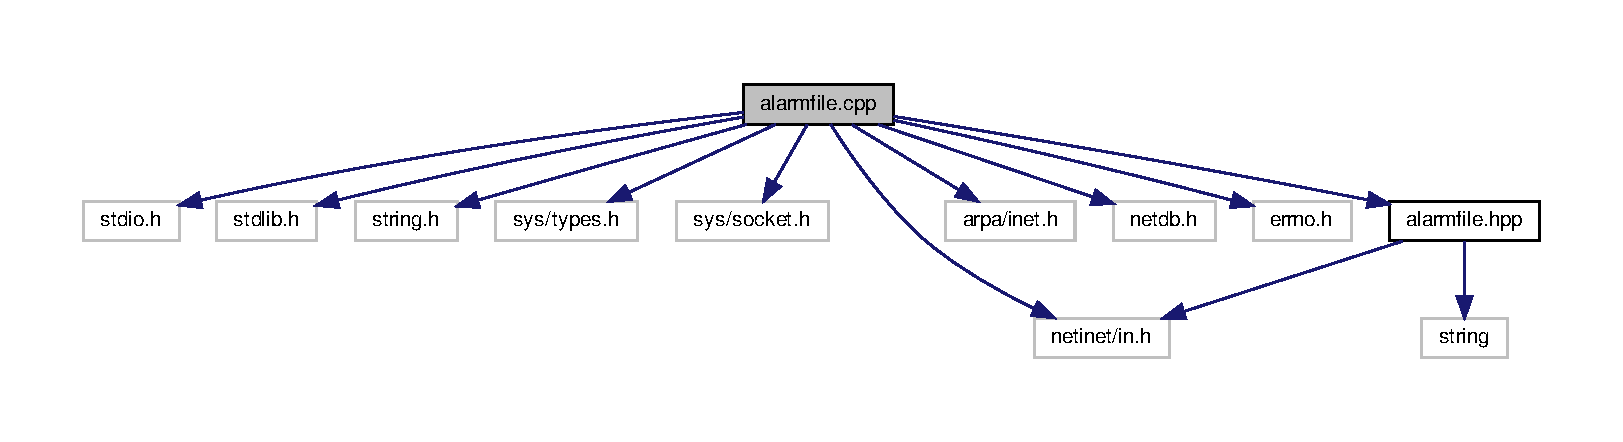
\includegraphics[width=350pt]{alarmfile_8cpp__incl}
\end{center}
\end{figure}


\subsection{Descripción detallada}
Archivo que contiene la definición de la clase para la configuración y envío de un mensaje a un servidor remoto. 

\begin{DoxyAuthor}{Autor}
Juan Manuel Vozmediano Torres 
\end{DoxyAuthor}
\begin{DoxyDate}{Fecha}
09/04/2019 
\end{DoxyDate}


Definición en el archivo \hyperlink{alarmfile_8cpp_source}{alarmfile.\+cpp}.

